\documentclass[11pt,a4paper]{article}
\usepackage[margin=1in]{geometry}
\usepackage[T1]{fontenc}
\usepackage[utf8]{inputenc}
\usepackage{lmodern}
\usepackage{hyperref}
\usepackage{enumitem}
\usepackage{xurl}
\usepackage{tikz}
\usepackage{float}
\usetikzlibrary{arrows.meta, positioning, shapes.geometric}
\hypersetup{colorlinks=true,linkcolor=blue,urlcolor=blue}
\newcommand{\codepath}[1]{\path{#1}}
\tikzset{box/.style={rectangle,draw,rounded corners,align=center,inner sep=3pt,minimum width=36mm},decision/.style={diamond,draw,aspect=2.1,align=center,inner sep=2pt},line/.style={-Latex}}

\title{Phase-1 Deliverable: Validation Suite}
\author{SIT Engine Architecture}
\date{\today}

\begin{document}
\maketitle

\section{Technical Description}
Validation Suite enforces semantic correctness using invariant checks and golden replay over pinned datasets.

For Phase-0 parity context, validation also includes Wormhole-oriented checks from the Tenstorrent baseline workflow.

\section{Implementation Fulfillment}
Implemented through \codepath{Phase-1/tests/check_invariants.py} and \codepath{Phase-1/tests/run_golden_suite.py}. Optional deeper diagnostics exist in \codepath{Phase-1/tools/validation/validate.py} (Wormhole-target range checks). CI gate runs golden suite through \codepath{.github/workflows/phase1-ci.yml}.

\subsection*{Phase-0 Baseline Provenance (Verified)}
\begin{itemize}[leftmargin=*]
  \item Source repo: \url{git@github.com:Srinidhi-Magesh08/Tenstorrent_test_raw_files.git}
  \item Baseline branch/commit: \texttt{main} @ \texttt{4512ce4e1a689f64c866160bf1f8e7e5e3e2ec89}
  \item Baseline run artifact consumed for parity context: \codepath{phase0_golden/tt_run_2026-02-09/raw_profiler/profile_log_device.csv}
  \item Run header baseline: \texttt{ARCH=wormhole\_b0}, \texttt{CHIP\_FREQ[MHz]=1000}, \texttt{Max Compute Cores=64}
\end{itemize}

\section{Design \& Architecture}
The harness runs base and residency-mask modes per trace, executes invariant predicates, aggregates failures, and returns non-zero status on semantic drift. Manifest checks are strict (missing traces/masks fail the run), and the pinned set includes a Wormhole-derived Phase-0 sample trace in addition to synthetic regression traces.

\subsection*{Function Flowchart}
\begin{figure}[H]
\centering
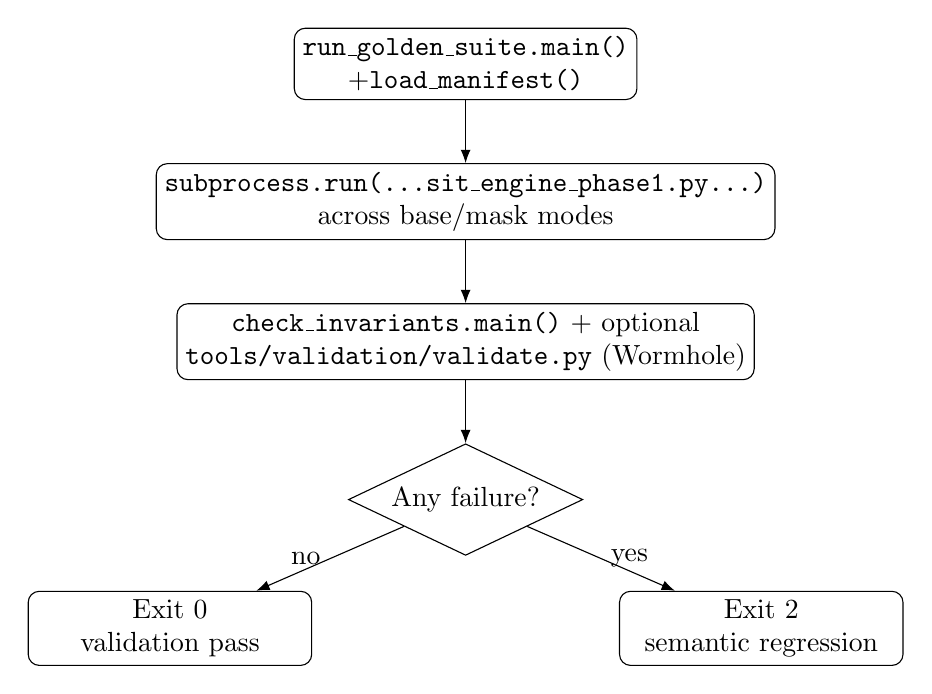
\begin{tikzpicture}[node distance=8mm and 12mm]
\node[box] (a) {\texttt{run\_golden\_suite.main()}\\+\texttt{load\_manifest()}};
\node[box, below=of a] (b) {\texttt{subprocess.run(...sit\_engine\_phase1.py...)}\\across base/mask modes};
\node[box, below=of b] (c) {\texttt{check\_invariants.main()} + optional\\\texttt{tools/validation/validate.py} (Wormhole)};
\node[decision, below=of c] (d) {Any failure?};
\node[box, below left=of d] (e1) {Exit 0\\validation pass};
\node[box, below right=of d] (e2) {Exit 2\\semantic regression};
\draw[line] (a) -- (b);
\draw[line] (b) -- (c);
\draw[line] (c) -- (d);
\draw[line] (d) -- node[left]{no} (e1);
\draw[line] (d) -- node[right]{yes} (e2);
\end{tikzpicture}
\caption{Validation Suite Function Flow}
\end{figure}

\end{document}
